\documentclass[a4paper]{article}
% generated by Docutils <http://docutils.sourceforge.net/>
\usepackage{fixltx2e} % LaTeX patches, \textsubscript
\usepackage{cmap} % fix search and cut-and-paste in Acrobat
\usepackage{ifthen}
\usepackage[T1]{fontenc}
\usepackage[utf8]{inputenc}

\usepackage{graphicx}
\usepackage{xcolor}

\usepackage{hyperref}

\newcommand{\tag}[1]{
\sffamily
\fcolorbox[RGB]{200,192,144}{200,248,200}{\textbf{#1}}
\normalfont
}

\newcommand{\ie}{{\textit{i.e.\ }}}
\newcommand{\cf}{{\textit{cf\ }}}
\newcommand{\eg}{{\textit{e.g.\ }}}



%%% Title Data
\title{Towards a new intermediate layer for geometric and temporal reasoning}
\author{Séverin Lemaignan et al.}
\date{}


%%% Body
\begin{document}
\maketitle


\section*{Report overview}

This report is organized as follow:

\begin{itemize}
    \item first, we present in broad terms the problem we try to solve,
    \item  then, we present a set of use-cases that underline the limitation of our current tools and hint to the new capabilities we want to endow our robots with,
    \item from these use-cases, we isolate a set of expected features for the software system we want to design,
    \item the fourth section present a short review of existing art,
    \item we present in the next section a set of early designs and proposals from the last year of discussions on this subject
    \item finally, we present the {\tt libworlds} proposal, as a synthesis attempt of the previous ideas.
\end{itemize}

\clearpage
%___________________________________________________________________________

\section{Problem Statement}
\label{problem-statement}%

In the stack of software components required for an autonoumous robot, the
layer that provide an uniform representation of the robot's environment not
only suitable, but even convenient for decision making, is crucial.

Because both the sensors inaccuracies and the dynamic nature of the world
(objects and structures constantly appear and disappear), this layer needs to
accomodate unexpected changes and filter out as much noise introduced by faulty
perception as possible, which also require the maintainance of an history of
the successive world states.

Also, this layer must remain as light as possible for the client layers.
These upper layers include components for geometric reasoning, temporal
reasoning/action recognition, geometric motion planner, symbolic task planners
(that need to control the geometric feasability of a plan), learning modules
and maybe others.

Figure~\ref{fig|saphari} gives a real world example of a (proposed)
architecture for a modern, interactive robot, from the SAPHARI project.

\begin{figure}[!h]
    \centering
    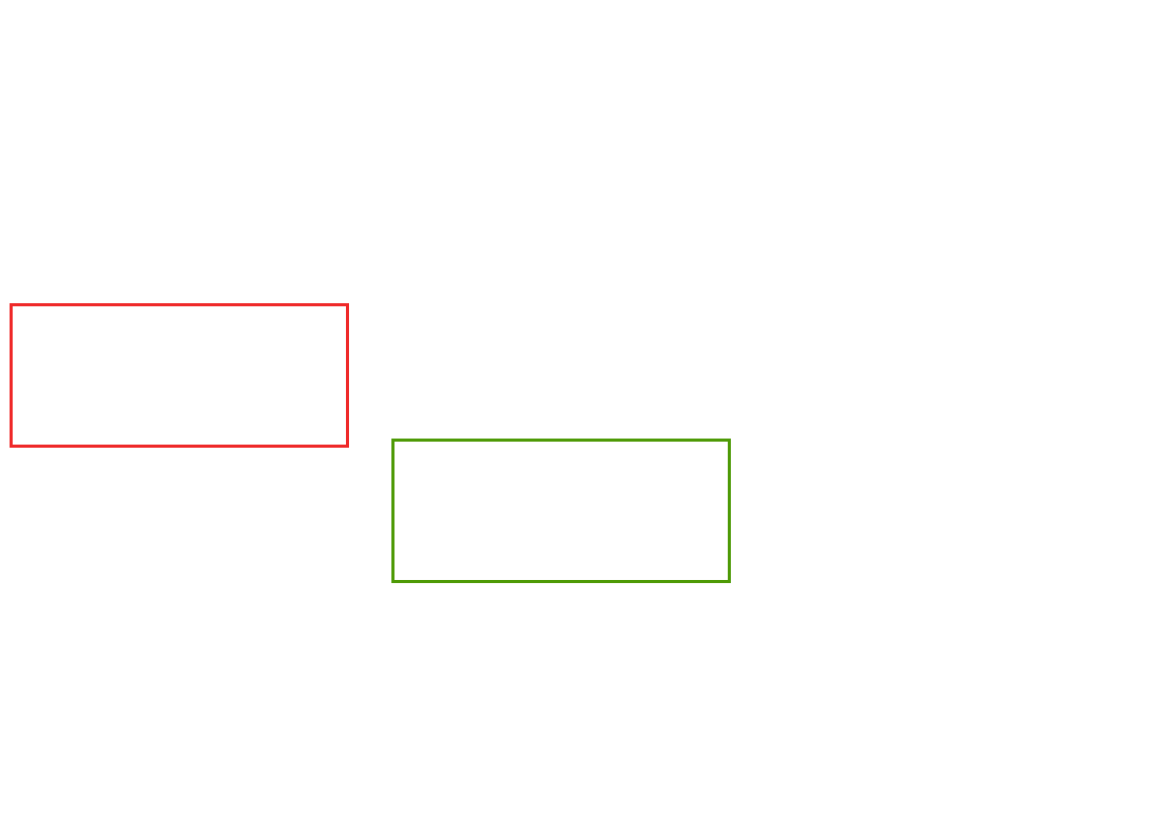
\includegraphics[width=\columnwidth]{images/saphari-focused.pdf}

    \caption{Draft of a proposed architecture for the European SAPHARI project.
    This proposal must enable a convenient and performant implementation of the
    functions in the red block, based on inputs from the green block.}

    \label{fig|saphari}
\end{figure}


The geometric and temporal representation layer is only an intermediate tool
used by higher cognitive functions: it must be light, convenient, performant.
The less we think about it, the better.

This does not mean it does a simple job. Amongst the challenging tasks we have
identified, we can mention:

\begin{itemize}
    \item ensuring physically realistic model of the world

    \item managing several level of refinement of object's model (from partial
        point clouds to accurate CAD models)

    \item managing plausible states for unseen/not visible objects
        (probabilistic modeling, physics reasoning)

    \item managing world discontinuities (eg, one single blob turns out to be
        two different objects, next to each other)

    \item representing suppositions (\eg a human tells the robot that a box is behind him)

    \item representing fields (\eg the field of reachability of an object for an agent)

\end{itemize}

Even if some of these tasks are not achieved in the first versions of the
project, we want to develop a software architecture that make it possible to
implement at some point this kind of features.

\subsection{Expected features}

\subsubsection{Temporal reasoning}

\begin{itemize}
    \item Many properties need to be assessed on a short time frame.
        SPARK must offer an easy way to access to delayed and/or
        filtered geometric properties of the scene.

    \item Idea of sliding time windows to monitor certain states, that
        could be dynamically modified (length, granularity...) 

\end{itemize}

\subsubsection{Alteration of the 3D model based on geometric reasoning}

corresponding use case: case 2 case 5

The outcomes of the reasoning should be possibly used to alter the 3D
model. For instance: a box is computed to be on another one, but perception
returns boxes are partially overlapping. SPARK should be able to update a
consolidated 3D model of the environment. 

\subsubsection{Good modularity/extensibility}

Two very different functions are fulfilled by the original SPARK: '''environment building and maintenance''' and '''geometric reasoning'''.

This two aspects are likely to be divided into 2 different modules in coming version. For convenience, requirements for both aspects are described here.


\begin{itemize}
    \item Plugin-based: each property is a plugin, i.e. a stand-alone
        library dynamically loaded with dlopen. This would allow to
        quickly add/remove computations

    \item ROS Nodelets? 

\end{itemize}



\section{Prior art}


\subsection{GSM}
\label{sect|gsm}

GSM (for \emph{Grounded Situation Model})~\cite{Mavridis2006} is a knowledge
representation system primarily built to ``facilitate cross-modal
interoperability'',  especially in the context of verbal interaction with a
robot.

GSM does not rely on any formal language but rather on a layered data structure
(figure~\ref{fig|gsm}) that organises the surrounding world into agents and
relations between agents.  Each agent (any animate or inanimate object) is
attached to a physical model (made of \emph{body parts} that have properties
like their position, color, etc.) and a mental model (which is a recursively
embedded GSM, thus allowing a sort of theory of mind).

\begin{figure}[!h]
    \centering
    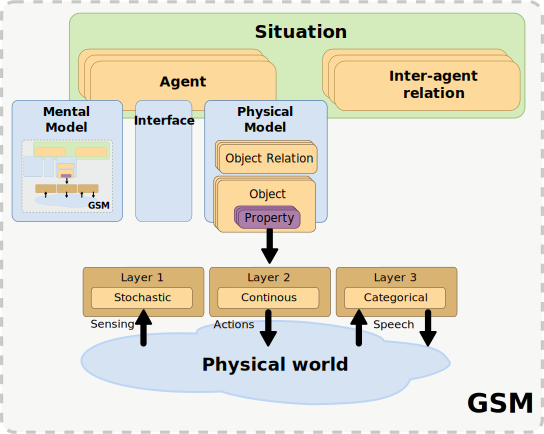
\includegraphics[width=0.65\columnwidth]{images/gsm.pdf}

    \caption{Simplified hierarchical structure of the Grounded Situation Model,
    based on~\cite{Mavridis2006}.}

    \label{fig|gsm}
\end{figure}

Properties are represented in three layers: a stochastic representation, close
to sensory percepts, a \emph{continuous single-valued} encoding of the
stochastic model, and a discrete, categorical model.

One notable feature of GSM is the \emph{bidirectionality} of the grounding
process: not only sensor percepts are abstracted into categories suitable for
human conversation, but human utterance (like ``There is a red ball in the
center of the table'') can also be turned into property descriptions. This
basically enable the knowledge representation system of the robot to
\emph{imagine} entities.

GSM also features several strategies for managing time and events.
\emph{Moments} are created by storing timestamped snap-shots of GSM, and
\emph{event classifiers} allow to define and detect events.

\paragraph{Experiments} GSM has mostly been tested on table-top manipulation
and interaction tasks (a ``conversational helping hand'' as stated by the
authors) implemented on a 7-DOF arm equipped with force feedback, cameras for blob
tracking and speech recognition (Sphinx4). Mavridis and Roy provide in addition
an in-depth analysis of the performance of GSM by the mean of a standard
psycholinguistic test, the \emph{Token test}~\cite{DiSimoni1978}.


\subsection{DyKnow}


%___________________________________________________________________________

\section{Use-cases}
\label{use-cases}%

For each case, labels indicates which aspect are involved: \tag{world building}, \tag{geometric reasoning}, \tag{temporal reasoning}

%___________________________________________________________________________

\subsection*{
  Case 1: an object is not perceived anymore, but stays in the model and ``floats in the air''%
  \label{case-1-an-object-is-not-perceived-anymore-but-stays-in-the-model-and-floats-in-the-air}%
}

\tag{world building}
%
\begin{quote}
%
\begin{itemize}

\item '''Option 1''': We want the object position to be filtered based on physical constraints (like gravity, or possible trajectory - taking into account previous speed)

\item '''Option 2''': {[}...?{]}

\end{itemize}

\end{quote}


%___________________________________________________________________________

\subsection*{
  Case 2: an agent grasps an object. The object is not visible anymore%
  \label{case-2-an-agent-grasps-an-object-the-object-is-not-visible-anymore}%
}

\tag{world building}
\tag{geometric reasoning}
%
\begin{quote}
%
\begin{itemize}

\item '''Option 1''': If we know the grasp was successful, then simply attach the object to the end effector

\item '''Option 2''': If we see again the object, far from the end effector, assume the grasp failed

\end{itemize}

\end{quote}

(cf also case 5)


%___________________________________________________________________________

\subsection*{
  Case 3: the perception routines are slightly unstable, objects keep moving around a bit%
  \label{case-3-the-perception-routines-are-slightly-unstable-objects-keep-moving-around-a-bit}%
}

\tag{world building}
%
\begin{quote}
%
\begin{itemize}

\item '''Option 1''': Implement proper dynamic filtering (low-pass filter)

\end{itemize}

\end{quote}


%___________________________________________________________________________

\subsection*{
  Case 4: the perception routines are strongly unstable, objects jump around%
  \label{case-4-the-perception-routines-are-strongly-unstable-objects-jump-around}%
}

\tag{world building}
%
\begin{quote}
%
\begin{itemize}

\item '''Option 1''': Implement proper geometric filtering, possibly coupled with physical simulation to check if a large displacement is actually physically possible

\end{itemize}

\end{quote}


%___________________________________________________________________________

\subsection*{
  Case 5: a object is perceived to be slightly INSIDE another one. Symbolic reasoning tells it is actually on top of it%
  \label{case-5-a-object-is-perceived-to-be-slightly-inside-another-one-symbolic-reasoning-tells-it-is-actually-on-top-of-it}%
}

\tag{world building}
\tag{geometric reasoning}
%
\begin{quote}
%
\begin{itemize}

\item '''Option 1''': Geometric reasoning should be allowed to provide feedback to the filtering routines to alter the model based on reasoning (cf also case 2)

\end{itemize}

\end{quote}


%___________________________________________________________________________

\subsection*{
  Case 6: the robot wants to predict ``what happen if I drop this object''%
  \label{case-6-the-robot-wants-to-predict-what-happen-if-i-drop-this-object}%
}

Equivalent use case: an object has disappeared, the robot wants to have ideas where to look for it.
\tag{geometric reasoning}
%
\begin{quote}
%
\begin{itemize}

\item '''Option 1''': Endow to robot with a physics engine that can be queried to compute possible positions for given objects in the future.

\end{itemize}

\end{quote}


%___________________________________________________________________________

\subsection*{
  Case 7: what is visible/reachable for each agents?%
  \label{case-7-what-is-visible-reachable-for-each-agents}%
}

\tag{geometric reasoning}
%
\begin{quote}
%
\begin{itemize}

\item '''Option 1''': As done in current SPARK, allow perspective taking.

\end{itemize}

\end{quote}


%___________________________________________________________________________

\subsection*{
  Case 8: the human says: ``there's a black box behind you''. The robot add it somehow%
  \label{case-8-the-human-says-there-s-a-black-box-behind-you-the-robot-add-it-somehow}%
}

\tag{geometric reasoning}
\tag{world building}

{[}this ability is called ''Presupposition Accommodation'': ability to assume a fact to be true, even without explicit prior knowledge. Cf \url{http://en.wikipedia.org/wiki/Presupposition\#Accommodation_of_presuppositions} and Mavridis2005{]}
%
\begin{quote}
%
\begin{itemize}

\item '''Option 1''': add support for presupposition accomodation (which implies the ability for the geometric reasoning to alter the world model)

\end{itemize}

\end{quote}


%___________________________________________________________________________

\subsection*{
  Case 9: the robot wants to go from A to B, but clutter on the ground prevent it. We want the robot to first remove hindering objects%
  \label{case-9-the-robot-wants-to-go-from-a-to-b-but-clutter-on-the-ground-prevent-it-we-want-the-robot-to-first-remove-hindering-objects}%
}

This use case requires external symbolic and geometric planing that is out of
the scope of SPARK. But SPARK should provide representations useful to solve
this kind of issue.


\section{Previous proposals}

In this section, we present the various ideas/proposals that have been designed
and discussed over the last year. Some of them are very early designs, and are
only useful to understand how the project evolved and refined itself over time.

\subsection{Continuous merging}

\begin{figure}[!h]
    \centering
    \includegraphics[height=10cm]{images/spark_archi0.png}
\end{figure}

One of the issues we often encounter when building a geometric model of the
robot environment is caused by perception inaccuracies: some objects are
floating around, in irrealistic ways (typically because they are suddently not
percieved anymore).

This early proposal introduce the idea of \textbf{physics-based reasoning} to
filter the geometric state: at each step, the future state (on ~100ms) of the
model is simulated by a physics engine, and we keep only the stable positions
of each entity.

\subsection{Cascading filters}

\begin{figure}[!h]
    \centering
    \includegraphics[height=10cm]{images/spark_archi1.png}
\end{figure}


In this architecture, a first module acquires and merge raw perception input,
and exposes the result as a "raw world state" poster/topic.

Then, a set of filters can be launched. They take one or several world model as
input and output a new, filtered, model. Amongst possible filters: a low-pass
one, another based on physics, etc.

Filters can be chained in any order, and can occur several times (for instance:
two low-pass filters, at different stage)

Finally, a special "geometric reasoning" module, that also act as a filter, is
in charge of computing symbolic facts from the geometric model.

It may embed its own physics engine for temporal projection ("what will happen
in the next 2 seconds if I drop the glass?") 

\subsection{"Timeline centric" Architecture proposal}

\subsubsection{Cascading filters}

The main idea is, similarly to the proposal ''Cascading filters'', to have a
set of cascading filtering modules that expose successive world models.

A first module merges into a 3D models several 3D positions sources (ROS TF
trees in the diagram below, but this can be discussed) and there corresponding
meshes (from URDF or Collada).

\begin{figure}[!h]
    \centering
    \includegraphics[scale=0.5]{images/spark2_archi2_1.png}
\end{figure}

This is very similar to what RVIZ does for instance.

However, it could be extended with temporal filters (like Kalman filter) to
merge several sources for the same info (like 2 Kinects tracking the same
human).

This first raw 3D world model is exposed and reused by several
stabilization/filtering modules:

\begin{figure}[!h]
    \centering
    \includegraphics[scale=0.5]{images/spark2_archi2_2.png}
\end{figure}

Each filter outputs a new world model. Other module can thus work with a world
model at any level of filtering.

In the diagram above, I've put some example of possible filters:

\begin{itemize}
    \item the \textbf{low-pass} filter aim at removing simple perception noise (shakiness)
    \item the \textbf{physics-based} filter uses a physics engine to:
        \begin{itemize}
            \item filter out impossible movements,
            \item ensure physical consistency (no floating objects, no object inside another one)
            \item account for movement of non-visible objects that can be physically deducted (like A is in B, B moves => A moves with B) 
        \end{itemize}

    \item the \textbf{symbolic reasoning} filter implement filtering at an even higher level, for instance:
        \begin{itemize}
            \item If A is perceived at 2 distinct places, then... there's an issue!
            \item See also Nico Blodow paper, page 4-5 for example of symbolic reasoning on a geometric model. 
        \end{itemize}
\end{itemize}

With this architecture, new filters can be later easily added.

\subsubsection{Timeline management}

This second proposal introduces the idea of a \emph{central timeline}. Every \emph{world
provider} (like filters) send to the timeline the changes:

\begin{figure}[!h]
    \centering
    \includegraphics[scale=0.5]{images/spark2_archi2_3.png}
\end{figure}

The timeline can be in turn used by other modules (like an \textbf{action
recognition} module) to know when a certain event occurred. The timeline
clients describe the kind of temporal event they are interested in (like "the
PR2 head moved twice in the last 3 mins), and get triggered when such an event
occurs:

\begin{figure}[!h]
    \centering
    \includegraphics[scale=0.5]{images/spark2_archi2_4.png}
\end{figure}

Cf below for details on the timeline events system.

\subsubsection{Reasoning on the world model}

The most stable world model can be used for various geometric reasoning tasks,
like perspective taking, geometric planing, simulation-based temporal
projection (cf paper by Lars Kunze, \cite{Kunze2011a}), etc.

\begin{figure}[!h]
    \centering
    \includegraphics[scale=0.5]{images/spark2_archi2_5.png}
\end{figure}

%___________________________________________________________________________

\section{
  The Worlds proposal%
  \label{the-worlds-proposal}%
}


%___________________________________________________________________________

\subsection{
  Overview%
  \label{overview}%
}

This document presents a software framework (temporarly) called libworlds that
aims to update the current tools for geometric reasoning in use at
LAAS, and support current and future researches in this field.

The softwares that we introduce here are \emph{low-level} with respect
to the \emph{reasoning} tasks: they do not implement any high-level
geometric and/or temporal reasoning algorithms. Instead, they
focus on offering efficient low-level libraries to \emph{store} and
\emph{query} geometric and temporal models of the world (known to the
robot).

The framework is build around the idea of \emph{worlds}: each world
contains a geometric \emph{model} built by the robot (from its
perceptions or from computation applied on other models) and a
\emph{timeline} associated to this model that allow to access the model
back and forth in time.


%___________________________________________________________________________

\subsection{
  Terminology%
  \label{terminology}%
}

We call \emph{state} a set of kinematic chains (made from 0 to n
joints) that describe a geometric and kinematic organisation of
rigid bodies. The structure of the states is described below.

We call \emph{Current Geometric State} (CGS) the latest state which
is directly built from the sensors. It represents the physical
world, as perceived by the robot.

We call \emph{event} the specific state where the set of conditions
described by the \emph{event pattern} attached to the event is computed
to become true.
The grammar of the event patterns is described below.

We call \emph{timeline} a linear datastructure that stores pairs of
(timestamp, state) each time one of the events registered with the
timeline is triggered.

We call a \emph{world} a tuple (state, timeline, repository of event
patterns)

We call \emph{Current World} the world that contains the \emph{Current Geometric State}.


%___________________________________________________________________________

\subsection{
  libworlds API%
  \label{libworlds-api}%
}

libworlds exposes four APIs:
%
\begin{itemize}

\item the \emph{worlds API} allows to create a new or access an existing
world. When creating a new one, it can possibly be initialised
from another, existing one, and becomes then completely
independent: if altered (for planing, prediction, filtering...),
it does not impact the original world.

The API also allow to compare, diff and merge worlds with each others.

\item the \emph{states API} allows to alter and access a geometric state in
an efficient, thread- and process-safe way. This API is the main
entry point for sensor inputs and filters.

\item the \emph{event API} allows to register new events pattern: these
patterns are checked against the world's state, and when they
trigger, the current state is stored in the timeline (actually,
only a diff is stored). Events can be hierarchical, and the
patterns can refer to other, already defined, events.

\item the \emph{timeline API} lets users retrieve the state of the world at
certain time points in the past (either absolute or relative to
past events), or possibly in the future if future states are
available (after planning, for instance).

\end{itemize}


%___________________________________________________________________________

\subsection{
  Use-cases and workflow examples%
  \label{use-cases-and-workflow-examples}%
}


%___________________________________________________________________________

\subsubsection*{\phantomsection%
  Sensor filtering%
  \addcontentsline{toc}{subsubsection}{Sensor filtering}%
  \label{sensor-filtering}%
}


%___________________________________________________________________________

\subsubsection*{\phantomsection%
  Planning%
  \addcontentsline{toc}{subsubsection}{Planning}%
  \label{planning}%
}


%___________________________________________________________________________

\subsubsection*{\phantomsection%
  Action recognition%
  \addcontentsline{toc}{subsubsection}{Action recognition}%
  \label{action-recognition}%
}


%___________________________________________________________________________

\subsubsection*{\phantomsection%
  Geometric reasoning and perspective-taking%
  \addcontentsline{toc}{subsubsection}{Geometric reasoning and perspective-taking}%
  \label{geometric-reasoning-and-perspective-taking}%
}


%___________________________________________________________________________

\subsection*{\phantomsection%
  Implementation%
  \addcontentsline{toc}{subsection}{Implementation}%
  \label{implementation}%
}


%___________________________________________________________________________

\subsubsection*{\phantomsection%
  Structure of states%
  \addcontentsline{toc}{subsubsection}{Structure of states}%
  \label{structure-of-states}%
}

A geometric state is stored as directed forests (a set of
directed graphs). Edges represent kinematic joints, while nodes
represent rigid bodies (soft bodies can not be represented in the
current state of this API).

Rigid bodies are represented as a structure containing:
%
\begin{itemize}

\item an unique identifier

\item their bouding boxes

\item a reference frame

\item a transformation matrix relative to the reference frame

\item the type of object (based on the robot ontology, default to ``Object'')

\item (optionally) a covariance matrix representing the uncertainty on the position and orientation of the body

\item (optionally) an (open) set of references to data representing the body (as described at the next section)

\end{itemize}

TBD: idea of fields (eg for Mightability Maps)?
TODO: very efficient wrappers for OpenGL and collision detection


%___________________________________________________________________________

\subsubsection*{\phantomsection%
  Bodies library%
  \addcontentsline{toc}{subsubsection}{Bodies library}%
  \label{bodies-library}%
}

In order to minimise the size of the worlds' states, all data used
to represent a body (parametric model, meshes, point-clouds) are
stored in an external database (SQL, NoSQL? TBD), shared by all
worlds.

Each record in this database contains:
%
\begin{itemize}

\item an unique identifier (egal to the SHA1 of the dataset)

\item a code specifying the type and format of the dataset (TBD)

\item the actual dataset

\end{itemize}


%___________________________________________________________________________

\subsubsection*{\phantomsection%
  Timeline and state diffs%
  \addcontentsline{toc}{subsubsection}{Timeline and state diffs}%
  \label{timeline-and-state-diffs}%
}

TBD


%___________________________________________________________________________

\subsubsection*{\phantomsection%
  Events patterns%
  \addcontentsline{toc}{subsubsection}{Events patterns}%
  \label{events-patterns}%
}

Cf Vincent


%___________________________________________________________________________

\subsection*{\phantomsection%
  Development road-map%
  \addcontentsline{toc}{subsection}{Development road-map}%
  \label{development-road-map}%
}

1. Implementation of the state API for a single world (the \emph{Current World}), including the \emph{bodies library} repository.
1bis. Development of a first client to load 3D meshes and kinematic chains (based on the ASSIMP library)
1ter. Development of a second client to display the state, based on TF and the existing visualisation capabilities of RVIZ.
\newcounter{listcnt0}
\begin{list}{\arabic{listcnt0}.}
{
\usecounter{listcnt0}
\addtocounter{listcnt0}{1}
\setlength{\rightmargin}{\leftmargin}
}

\item Support for NIUT and Viman
\end{list}

3. Development of another client that exports the state as a SPARK poster
3bis. Modification of SPARK to accept a world state from a poster

4. Development of OpenGL and collision detection wrappers (Bullet?)
4bis. Development of helpers to compute collisions
\setcounter{listcnt0}{0}
\begin{list}{\arabic{listcnt0}.}
{
\usecounter{listcnt0}
\addtocounter{listcnt0}{4}
\setlength{\rightmargin}{\leftmargin}
}

\item Integration with ROS's table-top detector to acquire meshes
\end{list}

6. Implementation of the events and timeline API
6bis. Development of an efficient diffing algorithm
\setcounter{listcnt0}{0}
\begin{list}{\arabic{listcnt0}.}
{
\usecounter{listcnt0}
\addtocounter{listcnt0}{6}
\setlength{\rightmargin}{\leftmargin}
}

\item Implementation of the Worlds API.

\item Port of SPARK situation assessment to libworlds.
\end{list}

\bibliographystyle{abbrv}
\bibliography{/home/slemaign/work/biblio/biblio_phd_severin}

\end{document}
